\section{Auswertung}
\label{sec:Auswertung}

\subsection{Zeitabhängigkeit der Amplitude}
\label{sec:Zeitabhängigkeit der Amplitude}

\begin{figure} [H]
  \centering
  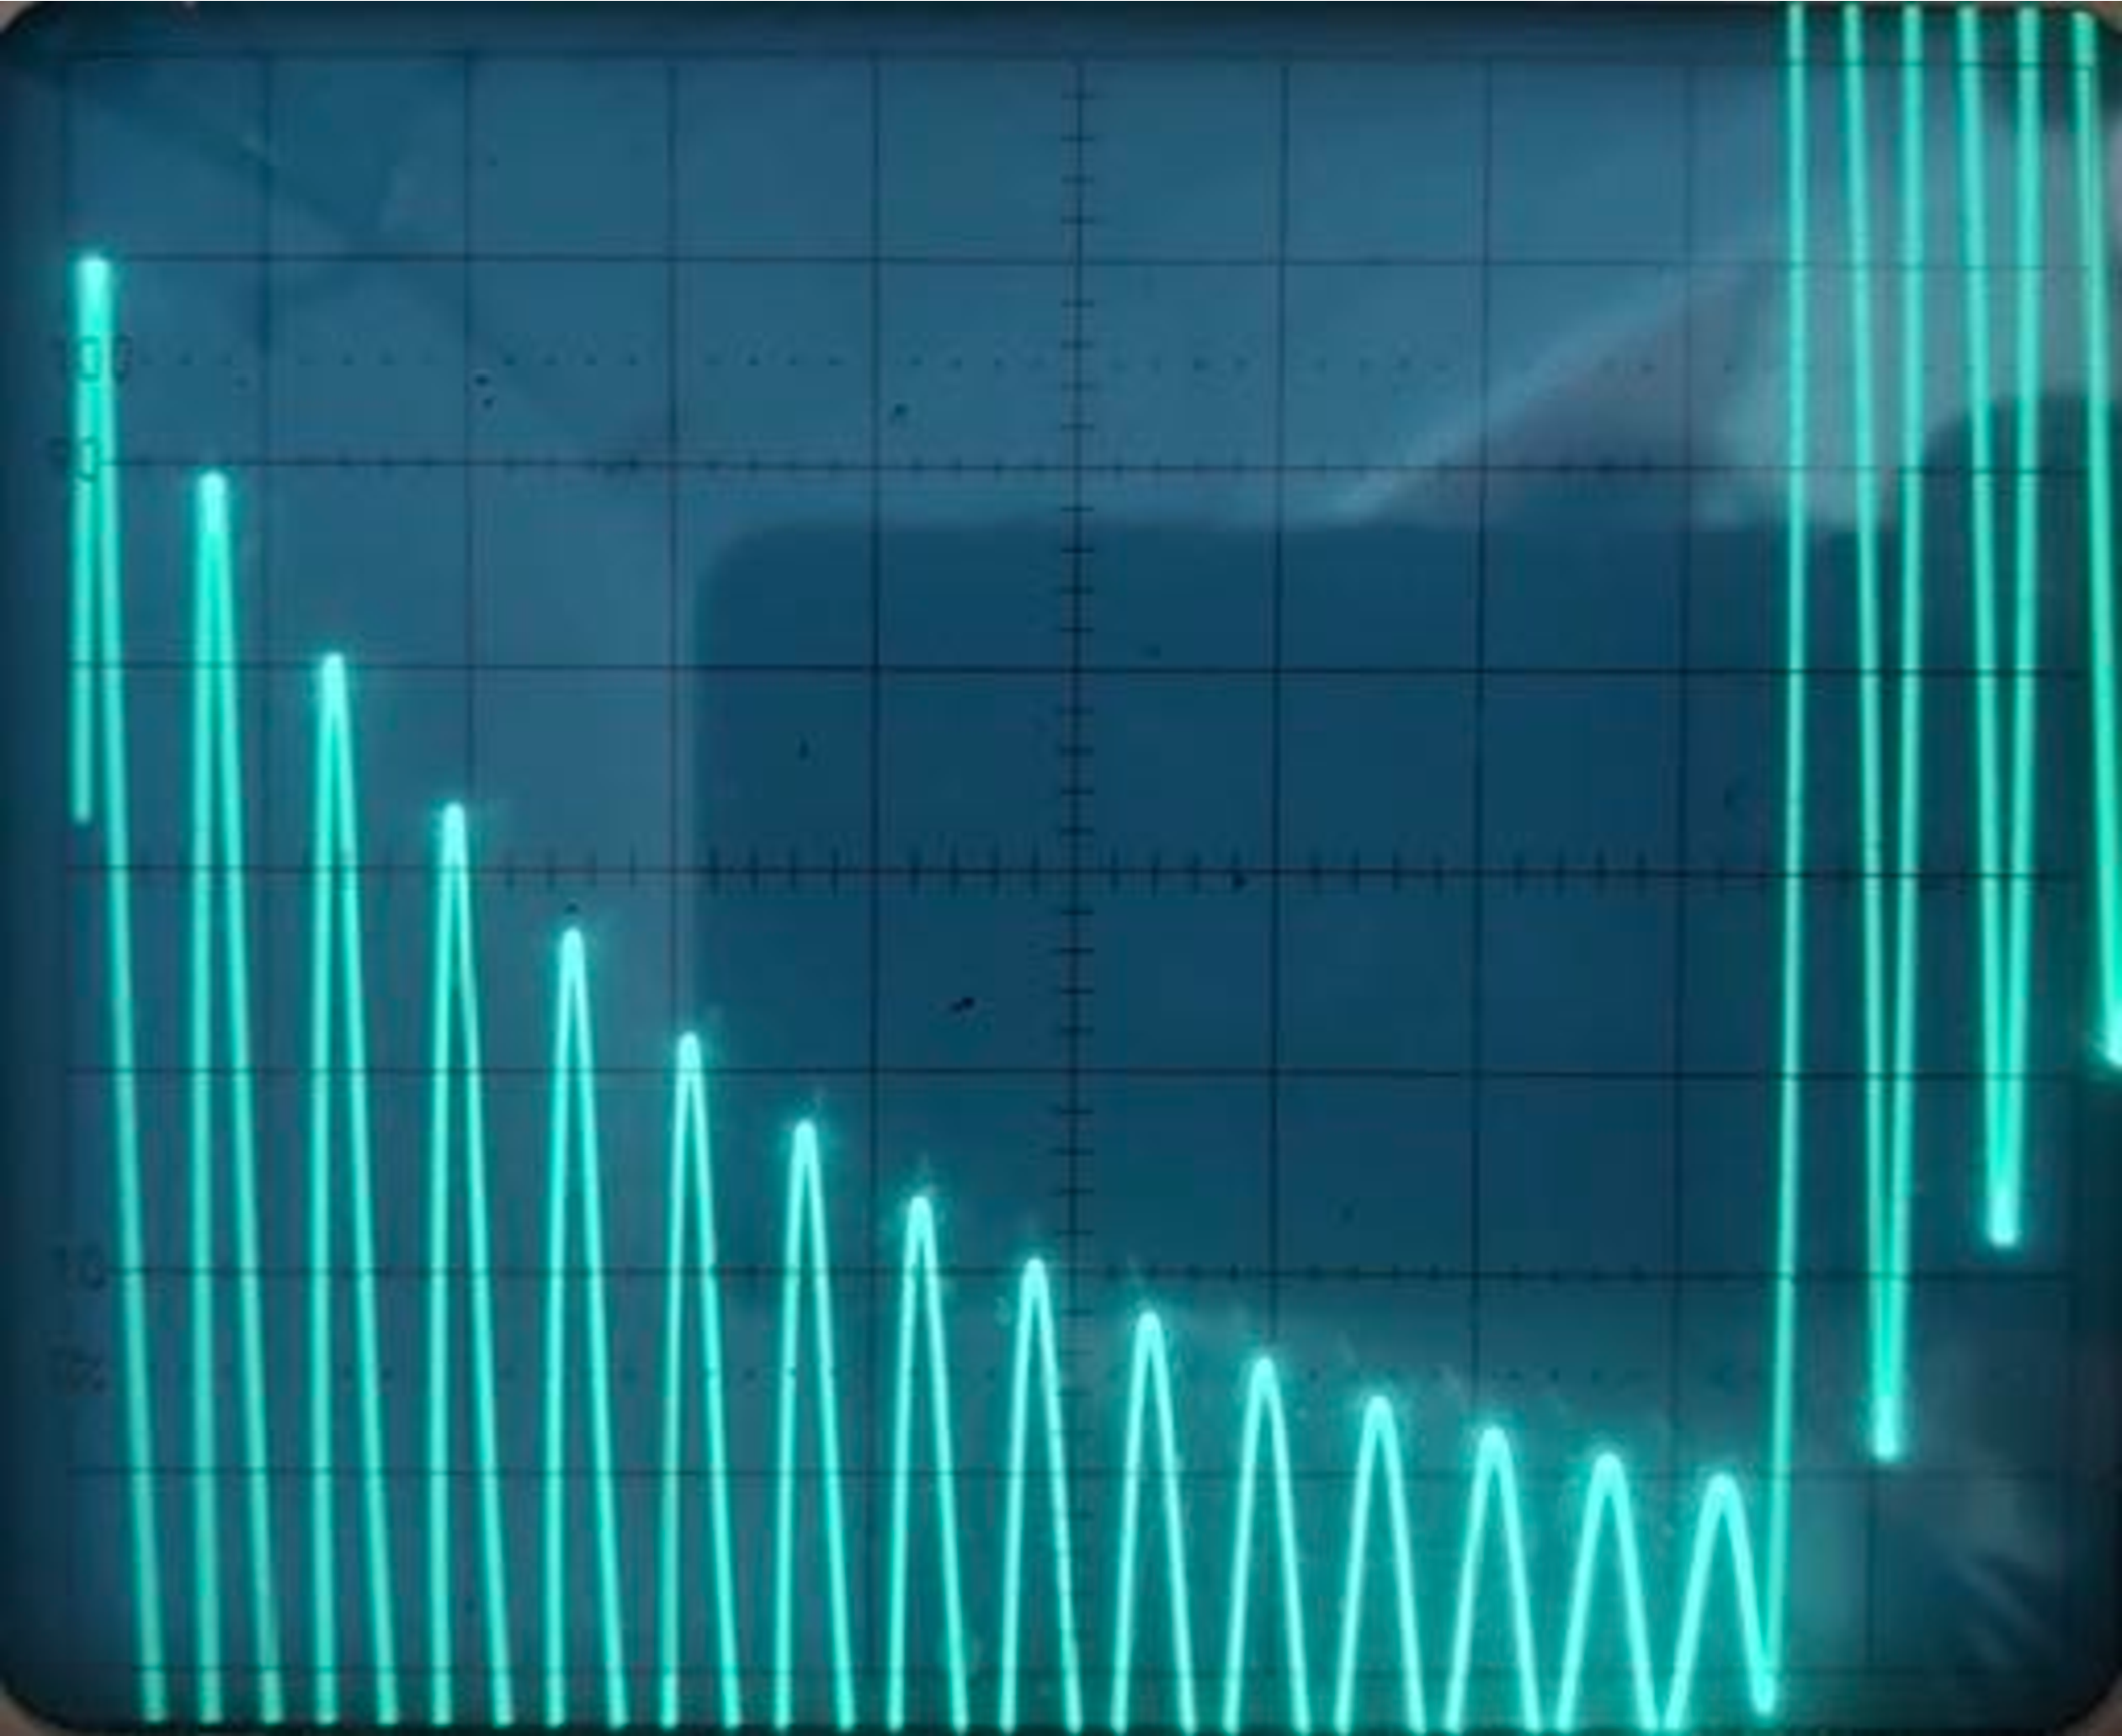
\includegraphics[height=10cm]{content/Bilder/Aufgabe_a.pdf}
  \caption{Bild des Oszilloskopbildschirms aus dem die Höhe der Amplituden der einzelnen Peaks abgelesen wird.}
  \label{fig:aufgabe a}
\end{figure}

Sagen, dass Abstand zwischen Peaks immer \qty{27,27}{\micro\second}
\begin{table}
  \centering
  \caption{Amplitude der einzelnen Peaks aus \autoref{fig:aufgabe a}.}
  \label{tab:Aufgabe a}
  \begin{tabular}{S[table-format=1.1]}
    \toprule
    {$U\,/\,\unit{\volt}$} \\
    \midrule
    6.0 \\
    5.0 \\
    4.1 \\
    3.3 \\
    2.7 \\
    2.2 \\
    1.8 \\
    1.4 \\
    1.1 \\
    0.8 \\
    0.5 \\
    0.4 \\
    0.2 \\
    0.1 \\
    \bottomrule
  \end{tabular}
\end{table}

\subsection{Frequenzabhängigkeit der Spannung}
\label{sec:Frequenzabhängigkeit der Spannung}

\begin{table}
  \centering
  \caption{Messwertpaare der zur Frequenz $f$ zugehörigen Amplituden $U_{0}$, $U$ sowie der Relativamplitude $\frac{U}{U_{0}}$.}
  \label{tab:Aufgabe c}
  \begin{tabular}{S[table-format=2.0] S[table-format=1.1] S[table-format=2.1] S[table-format=1.1]}
    \toprule
    {$f\,/\,\unit{\hertz}$} & {$U_{0}\,/\,\unit{\volt}$} & {$U\,/\,\unit{\volt}$} & {$\frac{U}{U_{0}}$} \\
    \midrule
    10 & 3.6 & 4.0  & 1.1 \\
    15 & 3.6 & 4.2  &	1.2 \\
    20 & 3.6 & 5.2  & 1.4 \\
    22 & 3.6 & 6.0  & 1.7 \\
    24 & 3.6 & 6.6  & 1.8 \\
    26 & 3.6 & 7.6  & 2.1 \\
    28 & 3.6 & 9.0  & 2.5 \\
    29 & 3.6 & 10.0 & 2.8 \\
    30 & 3.6 & 11.0 & 3.1 \\
    31 & 3.6 & 12.5 & 3.5 \\
    32 & 3.6 & 13.0 & 3.6 \\
    33 & 3.6 & 14.0 & 3.9 \\
    34 & 3.6 & 13.8 & 3.8 \\
    35 & 3.6 & 13.0 & 3.6 \\
    36 & 3.6 & 12.0 & 3.4 \\
    37 & 3.6 & 11.0 & 3.1 \\
    38 & 3.6 & 9.5  & 2.6 \\
    40 & 3.6 & 7.6  & 2.1 \\
    42 & 3.6 & 6.0  & 1.6 \\
    45 & 3.6 & 4.4  & 1.2 \\
    47 & 3.6 & 3.8  & 1.1 \\
    \bottomrule
  \end{tabular}
\end{table}

\begin{figure} [H]
  \centering
  \includegraphics{build/plot_c.pdf}
  \caption{Frequenzabhängigkeit der Spannung}
  \label{fig:plot_c}
\end{figure}

\begin{figure} [H]
  \centering
  \includegraphics{build/plot_c_2.pdf}
  \caption{Linearer Plot der Messwerte im Resonanzbereich}
  \label{fig:plot_c_2}
\end{figure}

\subsection{Frequenzabhängigkeit der Phasenverschiebung}
\label{sec:Frequenzabhängigkeit der Phasenverschiebung}

\begin{table} [H]
  \centering
  \caption{Messwertepaare der von der Frequenz $f$ abhängigen
  Phasenverschiebung $\varphi$, die aus dem Phasenversatz $a$ und der Periodenlänge $b$ berechnet wird.}
  \label{tab:aufgabe d}
  \begin{tabular}{S[table-format=2.0] S[table-format=1.1] S[table-format=2.0] S[table-format=1.3]}
    \toprule
    {$f\,/\,\unit{\hertz}$} & {$a\,/\,\unit{\micro\metre}$} & {$b\,/\,\unit{\micro\metre}$} & {$\varphi$} \\
    \midrule
    10 & 1.0 & 98 & 0.064 \\ 
    15 & 1.0 & 75 & 0.083 \\
    20 & 1.2 & 49 & 0.153 \\
    22 & 1.6 & 44 & 0.228 \\
    24 & 1.8 & 41 & 0.275 \\
    26 & 2.2 & 38 & 0.363 \\
    28 & 2.8 & 35 & 0.502 \\
    29 & 3.4 & 34 & 0.628 \\
    30 & 3.8 & 33 & 0.723 \\
    31 & 4.4 & 32 & 0.863 \\
    32 & 5.0 & 31 & 1.013 \\
    33 & 6.0 & 30 & 1.256 \\
    34 & 7.0 & 29 & 1.516 \\
    35 & 7.8 & 29 & 1.689 \\
    36 & 8.4 & 28 & 1.884 \\
    37 & 9.0 & 27 & 2.094 \\
    38 & 9.2 & 26 & 2.223 \\ 
    40 & 9.6 & 25 & 2.412 \\
    42 & 9.7 & 24 & 2.539 \\ 
    45 & 9.6 & 22 & 2.741 \\
    47 & 9.6 & 21 & 2.872 \\
    \bottomrule
  \end{tabular}
\end{table}

\begin{figure} [H]
  \centering
  \includegraphics{build/plot_d.pdf}
  \caption{Frequenzabhängigkeit der Phasenverschiebung}
  \label{fig:plot_d}
\end{figure}

\begin{figure} [H]
  \centering
  \includegraphics{build/plot_d_2.pdf}
  \caption{Linearer Plot der Messwerte im Bereich um $\frac{\pi}{2}$}
  \label{fig:plot_d_2}
\end{figure}